\documentclass[a4paper]{usiinfbachelorproject}

\captionsetup{labelfont={bf}}
\usepackage{float}
\usepackage{amsmath}
\usepackage{graphicx}
\usepackage{enumitem}
\usepackage{booktabs}
\usepackage{hyperref}

\author{POLAD BAKHISHZADE}

\title{\textbf{LLM as Code-Correctness Judge}}
\subtitle{Unveiling the Causes of Large-Language-Model Failures when Assessing Java Code}
\versiondate{\today}

\begin{committee}
  \advisor[Università della Svizzera italiana, Switzerland]{ }{Gabriele}{Bavota}
  \coadvisor[Università della Svizzera italiana, Switzerland]{ }{Giuseppe}{Crupi}
\end{committee}

% ——————————————————————————— ABSTRACT
\abstract{
\textbf{Context.}  
Large Language Models (LLMs) are increasingly being used in software development tasks such as code generation, explanation, and bug fixing. An emerging frontier is the use of LLMs for code review—specifically, assessing whether a given implementation is functionally correct. This requires reasoning over both the specification and the code, making it a strong benchmark for code understanding.\\
\\[2pt]
\textbf{Objective.}  
This study investigates how the quality and quantity of natural-language context affect the ability of LLMs to assess code correctness. We ask: \emph{What kind of descriptive information helps or harms the model’s ability to judge whether a function is correct?}\\
\\[2pt]
\textbf{Method.}  
We extend the Java subset of the \textsc{CoderEval} benchmark by systematically enriching it with five structured documentation layers—ranging from brief summaries to formal pre/post-conditions. Each of 362 functions is paired with one correct and one incorrect candidate implementation. We then prompt three open LLMs—Qwen-0.5B, Qwen-1.5B, and DeepSeek-1.3B—to act as zero-shot code judges, under multiple prompt configurations.\\
\\[2pt]
\textbf{Findings.}  
The results reveal that different models respond differently to added context: smaller models benefit from concise behavioral descriptions but often degrade when presented with verbose examples or formal constraints. In contrast, larger models leverage detailed descriptions to reduce mistakes and achieve more reliable judgments. Some layers, such as examples, can introduce confusion and accuracy drop depending on the model.\\
\\[2pt]
\textbf{Outcome.}  
The study highlights the importance of model-specific prompt design and shows that more documentation is not always better. These insights can inform future systems that rely on LLMs for code quality assessment.\\
\\[2pt]
\textbf{Keywords}: LLMs; Code Review; Code Correctness; Prompt Engineering; Evaluation; Java; Dataset Enrichment
}

\begin{document}
\maketitle
\tableofcontents\newpage

% ——————————————————————————— 1 INTRODUCTION
\section{Introduction}\label{sec:intro}
Large Language Models (LLMs) such as ChatGPT~\cite{openai2023chatgpt}, GitHub Copilot~\cite{githubcopilot}, and StarCoder~\cite{li2023starcoder} have become widely adopted in software development workflows. Originally developed for general language understanding, these models have rapidly gained traction in code-related tasks, including code generation, explanation, repair, and synthesis~\cite{jiang2024survey, chen2021codex, wang2023codet}. Researchers are increasingly exploring the use of LLMs for tasks such as debugging, static analysis, and functional correctness evaluation.\\
\\[2pt]
Among the many challenges in this space, one particularly important question is whether LLMs can serve as reliable evaluators of automatically generated code. In industrial settings, such as at Google, the proportion of code written or assisted by machine learning systems is steadily increasing. However, verifying the correctness of such code remains an open problem. Traditional techniques like writing unit tests are time-consuming and require substantial human effort, creating a bottleneck in workflows that rely heavily on automated code generation. Existing automatic evaluation metrics—such as BLEU~\cite{papineni2002bleu}, ROUGE~\cite{lin2004rouge}, METEOR~\cite{banerjee2005meteor}, and BERTScore~\cite{zhang2019bertscore}—have shown significant limitations in this setting. These metrics often rely on reference implementations, which may not be available, and struggle to capture functional equivalence between semantically correct but syntactically different solutions. Recent studies also highlight flaws in applying embedding-based metrics to code-related tasks~\cite{naik2024limitations}. This motivates the need for oracle-free evaluation mechanisms capable of assessing whether a candidate implementation adheres to a given specification.\\
\\[2pt]
While LLMs have shown strong performance in code generation, an open question remains: can they also reason about the correctness of code? This question has received relatively little attention so far, as most benchmarks are designed for code generation. Moreover, adapting code generation benchmarks for correctness evaluation is not trivial. Many such benchmarks provide only minimal or vague natural language descriptions, which are insufficient to test whether a model understands the functionality of the implementation it is evaluating.\\
\\[2pt]
In this work, we investigate how the judging abilities of LLMs vary with the depth and completeness of the instructions provided. Specifically, we create a correctness evaluation benchmark by extending the \textsc{CoderEval} dataset with five levels of natural language documentation. These range from a simple one-line summary of the function's purpose (L1), to a high-level description of the expected behavior and edge cases (L2), an explanation of the function signature and its parameters (L3), concrete input/output examples (L4), and formal pre- and postconditions specifying what must hold before and after execution (L5). We evaluate three instruction-tuned models—Qwen-0.5B, Qwen-1.5B, and DeepSeek-1.3B—across 362 function–candidate pairs. Each pair is tested under two conditions: \emph{cumulative prompts}, where the model sees all levels from L1 up to a given level, and \emph{ablation prompts}, where a specific level (e.g., L4) is removed from the full prompt to isolate its impact.\\
\\[2pt]
Our results suggest that the ability of LLMs to utilize different types of documentation varies across models. For instance, Qwen-1.5B shows a modest improvement in accuracy from 50\% to 55\% when provided with more detailed prompts, indicating some benefit from richer context. In contrast, smaller models like Qwen-0.5B and DeepSeek-1.3B exhibit inconsistent performance, sometimes declining with additional information. These findings suggest that prompt design can influence model performance, but its effectiveness varies: while richer prompts help some models slightly, others show inconsistent or even worse results.

\subsection*{Report structure}

Section~\ref{sec:related} reviews related literature.  
Section~\ref{sec:design} presents our study design and dataset enrichment pipeline.  
Section~\ref{sec:results} covers results from cumulative and ablation experiments.  
Section~\ref{sec:concl} concludes and outlines future directions.

% ——————————————————————————— 2 RELATED WORK
\section{Related Work}\label{sec:related}
As Large Language Models (LLMs) gain traction in software development, a growing body of research is investigating their potential not only as code generators but also as autonomous evaluators. Yet, assessing whether a model can reliably judge the correctness of code remains an open and challenging question. This section presents an overview of related efforts, focusing on the current limitations of LLM-based evaluation and recent benchmark development.\\
\\[2pt]
A key concern raised by recent work is that LLMs often lack deep semantic understanding of their own outputs. West et al.~\cite{west2023generative} formulate this as the “Generative AI Paradox”: models that generate impressive solutions may still fail to understand them. Their findings show that even top-tier LLMs frequently make overconfident yet incorrect predictions, especially on reasoning-intensive tasks. Gu et al.~\cite{gu2024counterfeit} expand this concern in the coding domain. They construct “counterfeit” solutions—plausible-looking but incorrect code—and show that LLMs often fail to flag these as erroneous. Instead, models are easily misled by surface-level cues and rarely recover from their own failures. Collectively, these studies highlight a core insight: evaluating code correctness is fundamentally distinct from generating code. Therefore, it is not safe to assume that a model which produces plausible-looking solutions is also a reliable evaluator of such completions.\\
\\[2pt]
Several studies have designed benchmarks to assess LLMs’ judgment ability in isolation. Zhao et al.~\cite{zhao2024codejudgeeval} introduce \textsc{CodeJudge-Eval}, a benchmark where LLMs must decide whether a given candidate solution is correct. The dataset includes subtle bugs, edge cases, and misleading code snippets. Across 12 models, including GPT-4 and Claude, accuracy remained low—rarely exceeding 60\%, with GPT-4 reaching at most 65\%. These results suggest that current models struggle with code correctness as a task, regardless of their size. Zhao et al. highlight that even advanced models like GPT-4 frequently misclassify incorrect solutions that contain subtle bugs or misleading logic. They suggest that reformulating the task—by giving more precise and complete descriptions of the expected behavior—and training models using datasets that include both correct and incorrect implementations could help improve judgment accuracy.\\
\\[2pt]
An influential approach is introduced by ICE-Score from Zhuo~\cite{zhuo2023icescore}, which suggests using GPT-3.5-turbo to evaluate candidate implementations using precisely crafted prompts that focus on properties such as correctness and readability. The study shows that prompting the model to explain its reasoning before delivering a final judgment enhances alignment with human evaluations.\\
\\[2pt]
Expanding on this idea, Tong and Zhang~\cite{tong2024codejudge} develop \textsc{CodeJudge}, a framework that builds on ICE-Score’s principles through a structured, multi-step evaluation process. In this setup, two instruction-tuned models are guided through reasoning stages—including explanation and justification—before returning a binary decision on correctness. Experiments reveal significant improvements in judgment accuracy across five datasets and programming languages, particularly for smaller models like Llama-3-8B-Instruct. In our study, we build on these insights but take a different angle: instead of structuring the reasoning steps, we structure the task description itself. By layering increasingly rich information—ranging from summaries to behavioral specifications and input/output examples—we investigate whether more detailed descriptions help models act as better judges.\\
\\[2pt]
While the studies above focus on correctness, others explore how to align model judgments with human coding preferences. Weyssow et al.~\cite{weyssow2024codeultrafeedback} introduce \textsc{CodeUltraFeedback}, a dataset of 10,000 coding problems, each answered by 14 different LLMs. These outputs are then ranked by GPT-3.5 across five dimensions: style, readability, instruction-following, complexity, and explanation. The authors use these rankings as training data to fine-tune CodeLlama-7B-Instruct, teaching it to prefer responses that GPT-3.5 rated more highly. The fine-tuned model is evaluated on HumanEval+~\cite{lzi2023humanevalplus}, where it outperforms the original base model in both preference alignment and functional accuracy. Although the task focuses on stylistic and qualitative assessment rather than functional correctness, the results suggest that training with ranked outputs can guide LLMs to better evaluate and generate code along desired dimensions such as style and readability.\\
\\[2pt]
A complementary line of research examines LLMs in educational settings. Koutcheme et al.~\cite{koutcheme2025evaluating} assess whether LLMs can generate and evaluate feedback on student code submissions in introductory Python assignments. Their goal is to explore how models can assist in automated grading systems that support student learning. They find that open-source models like StarCoder2 perform competitively with proprietary models such as GPT-4, particularly when provided with annotated student submissions that include instructor-written feedback, which serve as exemplars for what good feedback should contain. While not directly focused on correctness classification, this work supports the broader feasibility of using LLMs as evaluators of code quality.\\
\\[2pt]
In summary, the field is converging on the idea that LLMs can act as judges, but only under carefully crafted conditions. While prior work has focused on benchmarks, multi-step reasoning, or feedback alignment, our study lies in incrementally enriching the prompt descriptions and examining how models with different sizes respond to varying levels of contextual detail when judging code correctness.

% ——————————————————————————— 3 STUDY DESIGN
\section{Study Design}\label{sec:design}

\subsection*{Research Question}
\noindent\textbf{RQ –} \emph{To what extent does the quality and depth of natural language documentation affect the ability of LLMs to judge the correctness of a given Java function?}

\subsection{Context: LLMs}\label{sec:llms}
We selected three instruction-tuned large language models (LLMs) of relatively small size: \textbf{Qwen2.5-Coder-0.5B-Instruct}, \textbf{Qwen2.5-Coder-1.5B-Instruct}~\cite{qwen2024report}, and \textbf{DeepSeek-Coder-1.3B-Instruct}~\cite{deepseek2024report}. These models were chosen to balance performance and computational efficiency, enabling us to run multiple evaluation configurations on local hardware without relying on high-end GPUs or cloud infrastructure. Although computational cost was not a formal constraint of the study, using smaller models made experimentation more feasible and reproducible in standard academic settings.\\
\\[2pt]
All three models are optimized for code-related tasks and released with instruction-following tuning, meaning they have been fine-tuned to generate appropriate responses to structured natural language instructions. This makes them well-suited for prompt-based evaluation tasks like the one in this study.\\
\\[2pt]
The term \emph{“Instruct”} indicates that the model has undergone additional fine-tuning on datasets that include natural language prompts and desired completions, making it more responsive to task-specific queries. The Qwen models are part of Alibaba’s Qwen2.5 series, designed for code tasks and instruction-following scenarios. Qwen2.5-Coder models were trained on a large mixture of public and synthetic datasets, including a multilingual corpus of code, technical Q\&A, and structured programming tutorials~\cite{qwen2024report}. In particular, Qwen2.5-Coder-1.5B was optimized for multi-task code understanding and generation, and supports fine-grained control over function-level behavior through instruction tuning.\\
\\[2pt]
DeepSeek-Coder is a family of decoder-only transformer models specifically built for programming-related tasks~\cite{deepseek2024report}. The DeepSeek-Coder-1.3B variant used in our study was pre-trained on a massive 2 trillion token corpus that includes 87.5\% code and 12.5\% natural language. It was then instruction-tuned on 2 billion tokens of high-quality problem–solution pairs and user queries. The model supports over 80 programming languages and is explicitly optimized for tasks such as code completion, explanation, and functional verification, making it particularly suitable for prompt-based correctness evaluation.\\
\\[2pt]
All models were accessed via the Hugging Face Hub\footnote{\url{https://huggingface.co}}, an open-source platform that hosts pre-trained machine learning models and provides tools for deployment and evaluation. We used the Transformers library to run the models, which handled prompt tokenization, model loading, and inference (i.e., generating predictions) through a standardized API.

\subsection{Context: Dataset}\label{sec:dataset}
We based our experiments on the Java subset of the \textsc{CoderEval} benchmark~\cite{coderEval2023}, a code generation dataset containing 230 manually curated Java programming tasks. Each task includes: (i) a natural language specification describing what the function is expected to do, (ii) a reference implementation showcasing a possible correct solution, and (iii) an associated test suite for automated correctness verification.\\
\\[2pt]
Before adopting all 230 tasks, we performed a thorough quality assurance procedure to ensure the reliability of the test suites. This step was crucial, as test misbehavior could bias our evaluation—for instance, by incorrectly labeling an actually wrong solution as correct.\\
\\[2pt]
We discarded 49 problems for the following reasons:
\begin{itemize}[leftmargin=12pt]
  \item \textbf{20 tasks} had reference implementations that failed their own test suites.
  \item \textbf{9 tasks} had test suites so weak that even empty functions passed them.
  \item \textbf{17 tasks} passed with trivial dummy functions, e.g., \texttt{return null;} or \texttt{return 0;}, suggesting the test suite lacked discriminative power.
  \item \textbf{3 tasks} gave inconsistent test results for identical implementations.
\end{itemize}
This left us with a final set of 181 Java tasks, all of which passed our quality criteria and offered reliable correctness labels inferred directly from their test results.\\
\\[2pt]
Although each problem includes a natural language docstring, these descriptions are often minimal—typically consisting of one vague sentence. For instance:
\begin{itemize}[leftmargin=12pt]
  \item “This method returns a string.”
  \item “Calculate the result.”
\end{itemize}
Such documentation is insufficient for evaluating how LLMs understand code. Our goal was therefore to augment the dataset with rich, multi-layered natural language descriptions to enable a code understanding task, where LLMs must infer functional correctness from semantic cues.

\subsection{Data Collection}\label{sec:collection}

\subsubsection{Augmenting the Dataset}\label{sec:augmentation}
The goal of enrichment was to convert \textsc{CoderEval} from a code generation benchmark into one suitable for evaluating code understanding. Instead of asking models to generate code from a description, we wanted to test whether they could judge the correctness of a given implementation based purely on natural language documentation of the target function.\\
\\[2pt]
We used GPT-4o to produce this documentation because it was both scalable and accurate. Manual annotation of all 181 Java functions across multiple levels would have been impractical, and GPT-4o consistently followed structured formatting and stylistic constraints when prompted correctly.\\
\\[2pt]
Each prompt to GPT-4o included the full Java function body and its name. The model was asked to return a five-part structured description covering different semantic aspects of the function:

\begin{enumerate}[leftmargin=15pt]
  \item[\textbf{L1}] \textbf{Summary}: a concise one-sentence description of the function's high-level purpose, strictly excluding edge cases.
  \item[\textbf{L2}] \textbf{Behavioral description}: a 1--2 sentence narrative detailing the function’s logic, including how edge cases and special conditions are handled.
  \item[\textbf{L3}] \textbf{Signature explanation}: structured tags describing the meaning of each parameter and the return value (\texttt{@param}, \texttt{@return}, \texttt{@throws}), if applicable.
  \item[\textbf{L4}] \textbf{Examples}: several one-line input–output pairs with explanatory notes clarifying expected behavior.
  \item[\textbf{L5}] \textbf{Preconditions and postconditions}: short logical statements capturing required input constraints and expected output guarantees.
\end{enumerate}
The outputs followed a fixed format and were manually verified for quality and correctness. We ensured that L1 remained high-level, L2 captured the full logic and edge cases, and L3–L5 remained accurate, relevant, and specific to each function.\\
\\[2pt]
This enrichment gave us modular “building blocks” that could be flexibly combined into prompts with different levels of information. For example:
\begin{itemize}[leftmargin=12pt]
  \item \textbf{L1+L2}: A compact explanation of the function’s purpose and behavior.
  \item \textbf{L1+L3}: Purpose plus interface-level understanding, without relying on examples or logic.
\end{itemize}
This modularity was essential for constructing the incremental and layer-removal settings used in our evaluation.

\subsubsection{Building Candidate Pairs}\label{sec:judgments}
To evaluate whether LLMs can judge the functional correctness of code based on natural language descriptions, we paired each of the 181 Java functions with two candidate implementations: one correct and one incorrect. These implementations were not drawn from CoderEval itself, but were generated by us using several large language models, including DeepSeek-Coder-6.7B~\cite{deepseek2024report} and Qwen2.5-Coder-7B~\cite{qwen2024report}. We generated multiple candidate solutions for each function and compiled them into a custom knowledge base of over 5,000 Java implementations\footnote{\url{https://github.com/poladbachs/Bachelor-Thesis/blob/main/CoderEval/knowlbase_codereval.csv}}.\\
\\[2pt]
To ensure quality, we applied a filtering process to remove trivial, duplicate, or non-functional code. Specifically, we removed:
\begin{itemize}[leftmargin=18pt]
  \item Placeholder code, such as \texttt{/* implementation goes here */} or empty function bodies.
  \item Logic-less shells, including \texttt{return;} or \texttt{return 0;} with no computation.
  \item Print-only stubs like \texttt{System.out.println("TODO");}.
  \item Duplicates across the candidate pool.
  \item Candidates containing ambiguous or speculative language.
\end{itemize}
In particular, we discarded implementations containing the word \texttt{“assuming”}, such as:
\begin{itemize}[leftmargin=18pt]
  \item \texttt{// Assuming there's a getDefaultValue method for the class}
  \item \texttt{// Assuming IsomorphicGraphMapping is a custom class}
  \item \texttt{// Update heights (assuming that updateHeight() is defined)}
\end{itemize}
We excluded these because phrases like \emph{“assuming...”} indicate speculative dependencies on external structures, methods, or definitions not guaranteed to exist within the task context. Including such candidates would undermine our goal of evaluating implementations strictly based on the given information.\\
\\[2pt]
After cleaning, we finalized the dataset by selecting one correct and one incorrect implementation per function. When no valid correct candidate was found, we used the reference implementation from \textsc{CoderEval}. In two edge cases where no suitable incorrect candidate was available for a function, we manually inserted a faulty variant into the dataset to complete the correct–incorrect pairing.

\subsection{Prompting and Evaluation Setup}\label{sec:evaluation}
Each model was asked to solve the following binary classification task:

\begin{quote}
\emph{Given a natural language description and the signature of a target Java function, along with a candidate implementation, predict whether the implementation correctly satisfies the described functionality. Output \texttt{1} if it is correct, \texttt{0} otherwise.}
\end{quote}
The exact prompt given to the models was formatted as follows, using placeholders to insert task-specific information:

\begin{quote}\ttfamily
You will be provided with the description ("Description") and the signature ("Signature") of a Java function to implement. You will also see a candidate implementation ("Candidate"). Your role is to evaluate the correctness of the Candidate, providing as output either 0 or 1, and no other text:

0. Wrong Implementation: The implementation does not correctly implement the described function.\\
1. Correct Implementation: The implementation correctly implements the described function.

\# Description:\\
- Summary: \{L1: one-line summary\}\\
- Behavior: \{L2: behavioral explanation\}\\
- Signature Description: \{L3: @param/@return tags\}\\
- Examples: \{L4: input–output pairs with notes\}\\
- Preconditions and Postconditions: \{L5: logical constraints\}

\# Signature:\\
\{First line of candidate code\}

\# Candidate:\\
\{Full candidate implementation\}

\# Output:
\end{quote}
All prompts were encoded and passed to the models using Hugging Face Transformers with temperature set to 0.2 to reduce randomness and \texttt{max\_new\_tokens = 20}. A limit of \texttt{max\_new\_tokens = 20} was enforced to constrain output length and prevent verbose completions, as the task only required a single-digit response (0 or 1). Model outputs were parsed to extract a binary classification (\texttt{0} or \texttt{1}). Any output that did not conform to the expected format was treated as invalid and recorded as \texttt{None}.\\
\\[2pt]
We evaluated model performance under two experimental settings:

\paragraph{1. Prompt Enrichment.}
For each model, we incrementally increased the amount of documentation information provided in the prompt. The five enrichment levels were:
\begin{itemize}[leftmargin=15pt]
  \item \textbf{L1 only}: Summary of the function’s purpose.
  \item \textbf{L1 + L2}: Adds behavioral explanation with edge cases.
  \item \textbf{L1 + L2 + L3}: Adds signature-level tags.
  \item \textbf{L1 + L2 + L3 + L4}: Adds concrete input–output examples.
  \item \textbf{L1 + L2 + L3 + L4 + L5}: Full prompt including logical constraints.
\end{itemize}
This yielded 15 enrichment runs in total: 3 models × 5 levels each.

\paragraph{2. Layer Removal.}
We then conducted 8 additional runs where we removed specific documentation layers from the full prompt to isolate their impact. These configurations varied by model:
\begin{itemize}[leftmargin=15pt]
  \item For Qwen-0.5B, we performed 5 runs, each removing a single layer (L1 through L5) from the full prompt.
  \item For Qwen-1.5B, we tested the impact of removing L4 and L5 individually.
  \item For DeepSeek-1.3B, we ran 1 configuration without L5, motivated by prior observations of noise in that layer.
\end{itemize}
This dual-axis experimental design—incremental addition and targeted removal—enabled us to evaluate not only whether more documentation helps, but also whether certain kinds of documentation may hinder performance by introducing ambiguity or unnecessary detail.

\subsection{Data Analysis}\label{sec:analysis}
The models were tasked with binary classification: decide whether a given candidate implementation correctly matches the described function behavior.\\
\\[2pt]
To evaluate performance, we computed standard confusion matrix metrics—true positives (TP), true negatives (TN), false positives (FP), and false negatives (FN). Accuracy was used as the main metric:
\[
\text{Accuracy} = \frac{TP + TN}{TP + TN + FP + FN}
\]

We examined two experimental conditions:
\begin{enumerate}[leftmargin=15pt]
  \item[\textbf{(1)}] \textbf{Prompt enrichment:} For each model, we tracked how accuracy changed as we incrementally added documentation layers (L1, L1+L2, ..., L1–L5).
  \item[\textbf{(2)}] \textbf{Layer removal:} Starting from the full L1–L5 prompt, we removed one or more layers to observe their individual effect.
\end{enumerate}
For example, to test the effect of Examples (L4), we compared accuracy on L1–L5 vs. L1+L2+L3+L5. In some cases (e.g., DeepSeek), accuracy increased after removing L5, suggesting it introduced misleading constraints.\\
\\[2pt]Results were visualized via bar charts, allowing a direct comparison of model performance across prompt types. This analysis helped us understand not only how much context is helpful, but also which types of documentation may confuse smaller models.

\subsection{Replication Package}\label{sec:replication}
All source code, enriched datasets, model evaluation scripts, and plotting tools are available in the following GitHub repository:

\begin{center}
\url{https://github.com/poladbachs/Bachelor-Thesis}
\end{center}
The repository includes all CSVs, accuracy plots, confusion matrices, and detailed README instructions for full replication. Environment dependencies are specified in \texttt{requirements.txt}.

% ——————————————————————————— 4 RESULTS
\section{Results \& Discussion}\label{sec:results}

%------------------------------------------------------------------
\subsection{Incremental enrichment (L1 $\rightarrow$ L5)}
%------------------------------------------------------------------

\begin{figure}[H]\centering
  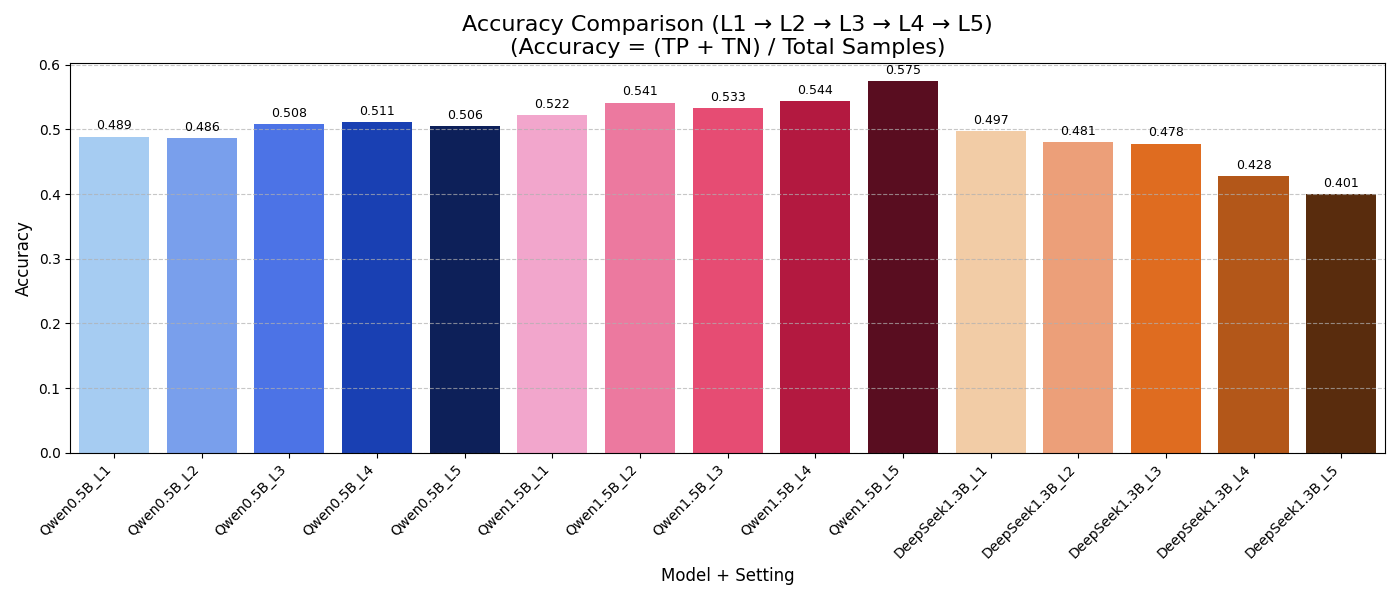
\includegraphics[width=0.95\linewidth]{figures/accuracy_comparison.png}
  \caption{Accuracy per model and documentation level.}
  \label{fig:acc-l1-l5}
\end{figure}

\paragraph*{Accuracy trends.}
We observe clear divergence in how each model responds to additional natural-language context:

\begin{itemize}[leftmargin=12pt]
  \item \textbf{Qwen-0.5B}: After stagnating on L1–L2, the model improves through L3 and L4, peaking at 0.511. L5 slightly degrades performance, suggesting diminishing returns or confusion from formal logic.
  
  \item \textbf{Qwen-1.5B}: Displays consistent benefit from each additional layer, rising steadily to 0.575 at L5. This model appears to handle verbosity well and leverages the full specification.

  \item \textbf{DeepSeek-1.3B}: Begins strong at 0.497 with minimal input, but drops with every added level—falling below 0.41 at L5. More context leads to worse performance, implying overload or poor instruction tuning for interpretive tasks.
\end{itemize}

These trends support our core hypothesis: smaller models benefit from concise cues, while larger models thrive on richer context. However, more detail is not universally helpful—its usefulness depends on model capacity and internal robustness to verbosity.

\vspace{0.8em}

% --------------------------- Qwen-0.5B
\begin{figure}[H]\centering
  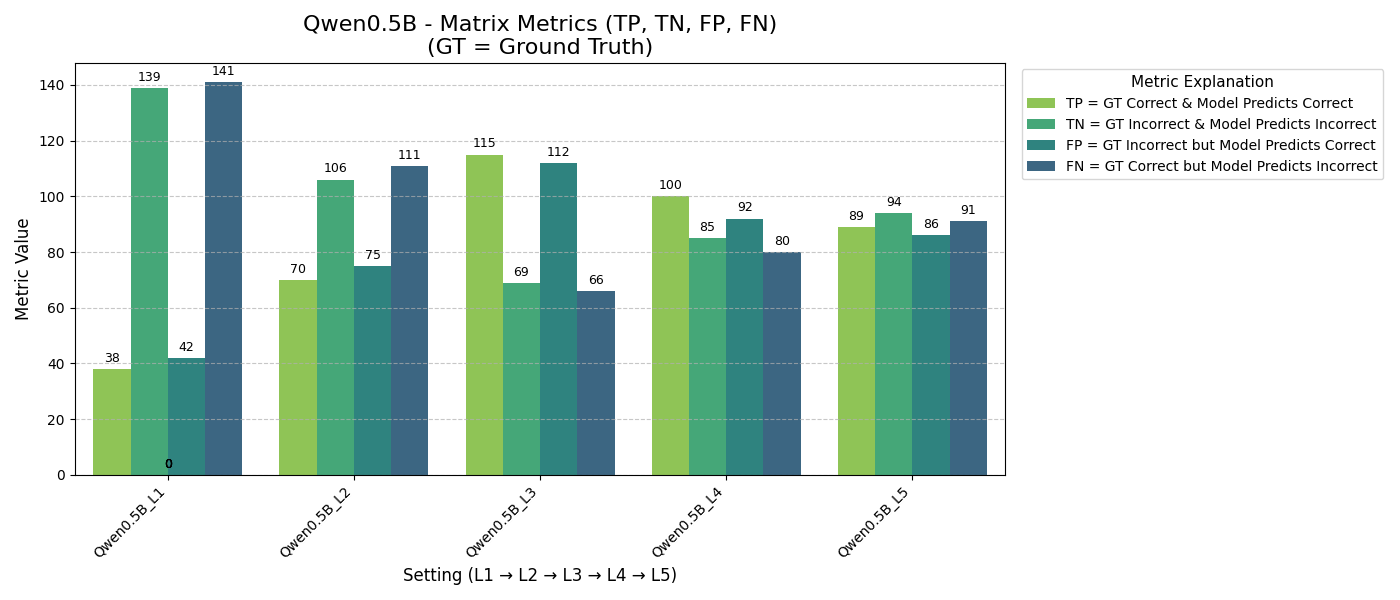
\includegraphics[width=\linewidth]{figures/Qwen0.5B_matrix_metrics.png}
  \caption{Confusion-matrix metrics — Qwen-0.5B.}
  \label{fig:q05-matrix}
\end{figure}

\paragraph*{Interpretation — Qwen-0.5B.}
Early stages (L1–L2) show a struggle to distinguish correct from incorrect implementations, with high false negatives. L3 and L4 reduce FN significantly, converting many correct cases into true positives. However, at L5 false positives creep back in, suggesting that formal conditions (pre/post) mislead the model or increase ambiguity. Overall, Qwen-0.5B needs concise clarity—too much structure destabilizes its judgment.

\vspace{0.8em}

% --------------------------- Qwen-1.5B
\begin{figure}[H]\centering
  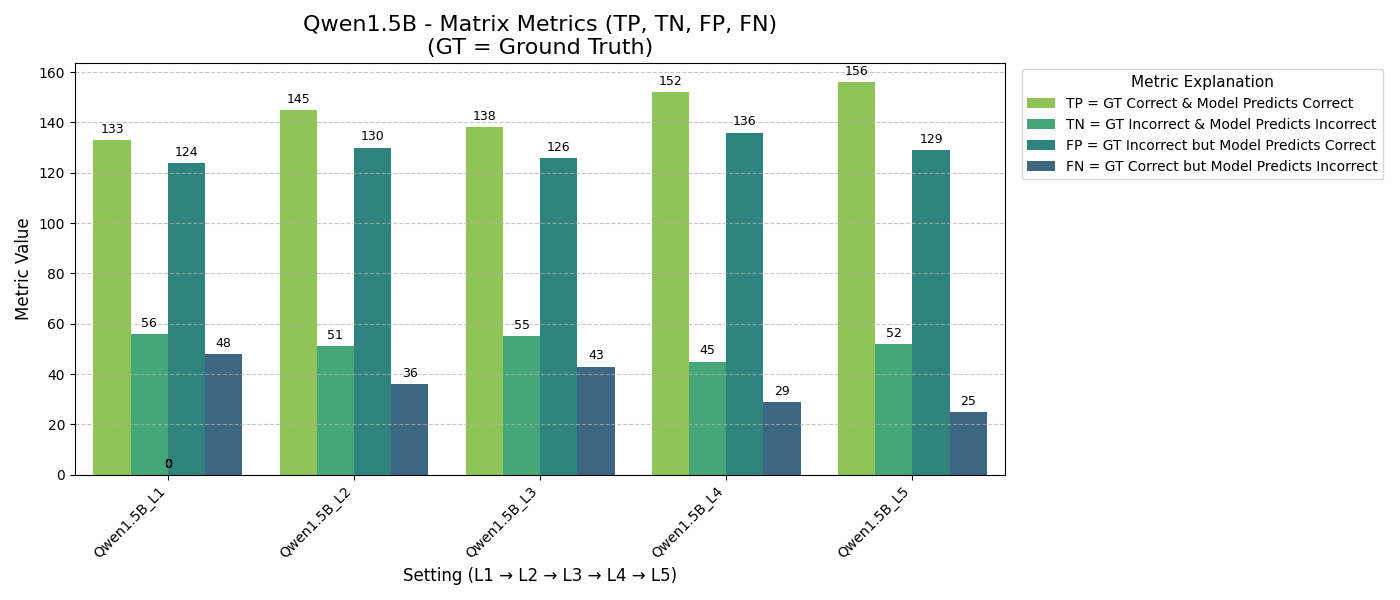
\includegraphics[width=\linewidth]{figures/Qwen1.5B_matrix_metrics.png}
  \caption{Confusion-matrix metrics — Qwen-1.5B.}
  \label{fig:q15-matrix}
\end{figure}

\paragraph*{Interpretation — Qwen-1.5B.}
The larger Qwen model handles incremental context with ease. As layers are added, false negatives drop sharply while true positives grow, especially after L4–L5. Pre/post-conditions help the model rule out wrong implementations without over-predicting correctness (FP stays stable). The balance between increased TP and maintained TN implies that Qwen-1.5B is the most context-aware model among the three.

\vspace{0.8em}

% --------------------------- DeepSeek-1.3B
\begin{figure}[H]\centering
  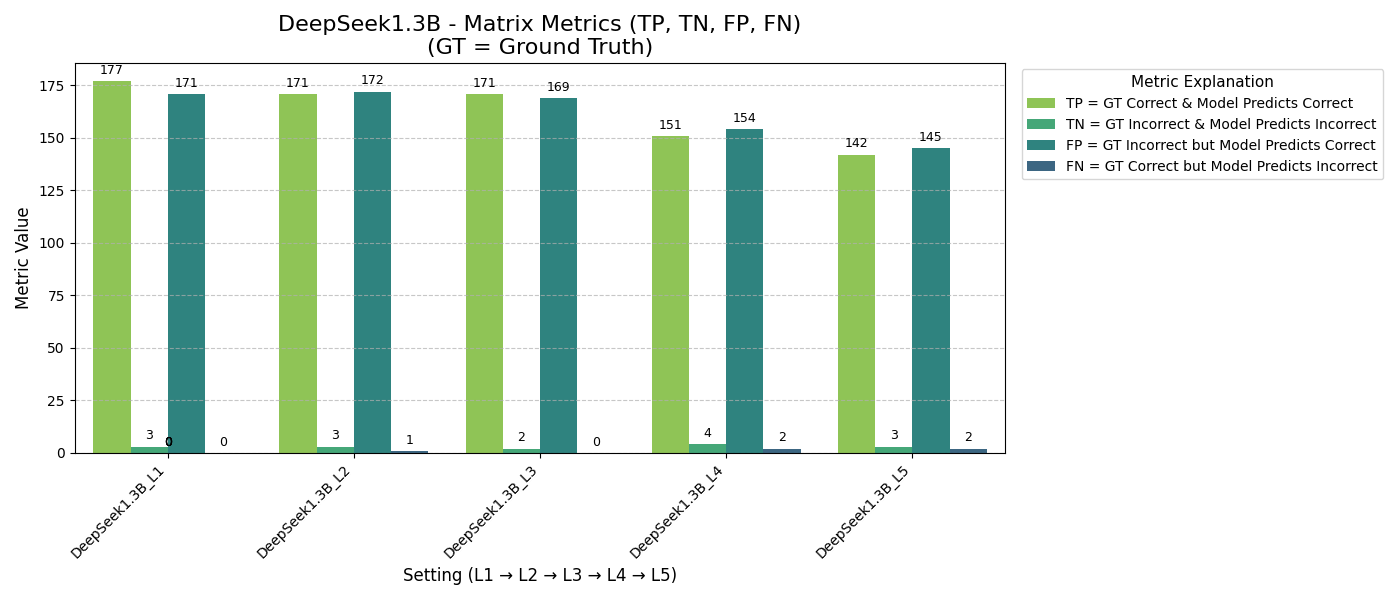
\includegraphics[width=\linewidth]{figures/DeepSeek1.3B_matrix_metrics.png}
  \caption{Confusion-matrix metrics — DeepSeek-1.3B.}
  \label{fig:ds-matrix}
\end{figure}

\paragraph*{Interpretation — DeepSeek-1.3B.}
Despite its comparable size, DeepSeek behaves like a brittle small model in judgment tasks. At L1 and L2, it achieves high TP with minimal FN. But starting at L3, false positives spike and true negatives collapse. This suggests that the added details—examples, constraints—shift attention away from core logic and confuse decision boundaries. It likely overfocuses on surface patterns in examples, falsely validating buggy code.



\subsection{Single-layer ablations}

\begin{table}[H]\centering
\caption{Accuracy after removing one layer. Values in parentheses show the change relative to the full prompt (L1--L5).}
\begin{tabular}{lccc}
\toprule
\textbf{Model} & \textbf{No L1} & \textbf{No L2} & \textbf{No L4} \\ \midrule
Qwen-0.5B  & 0.481 (–0.025) & \textbf{0.450 (–0.056)} & 0.494 (–0.012) \\
Qwen-1.5B  & 0.572 (–0.003) & 0.558 (–0.017) & 0.552 (–0.023) \\
DeepSeek-1.3B & \textbf{0.500 (+0.099)} & 0.434 (+0.034) & 0.428 (+0.028) \\
\bottomrule
\end{tabular}
\end{table}

\paragraph*{Interpretation.}
\begin{itemize}[leftmargin=12pt,itemsep=0pt]
  \item Removing behaviour (L2) cripples Qwen-0.5B (–5.6pp) $A \Rightarrow B$
 small model needs that layer.  
  \item Summary (L1) is useless or noisy for DeepSeek (+9.9pp when removed).  
  \item Qwen-1.5B tolerates all removals ($\leq$2pp), showing robustness.
\end{itemize}

\subsection{Compound ablations (illustrative)}

For space we discuss one illustrative combo per model:

\begin{itemize}[leftmargin=12pt]
  \item \textbf{Qwen-0.5B No L1 \& No L4}: accuracy 0.506 (–0.006 vs. full) — removing summary offsets example noise.  
  \item \textbf{Qwen-1.5B No L1 \& No L4}: 0.558 (–0.017) — examples help this model.  
  \item \textbf{DeepSeek No L2 \& No L4}: 0.478 (+0.078) — minimal prompt is best.  
\end{itemize}

\subsection{What makes a layer “noisy”?}
Manual error analysis highlights three patterns:

\begin{enumerate}[label=\alph*),leftmargin=15pt,itemsep=0pt]
  \item \textbf{Example bias}.  L4 lists only happy-path cases → model over-predicts “correct”.  
  \item \textbf{Narrative redundancy}.  L2 restates corner cases differently from L5, confusing alignment.  
  \item \textbf{Generic summaries}.  L1 adds little entropy; for DeepSeek it seems to trigger a “looks plausible → correct” bias.
\end{enumerate}

% ——————————————————————————— 5 CONCLUSIONS
\section{Conclusions \& Future Work}\label{sec:concl}

\begin{itemize}[leftmargin=12pt]
  \item Moderate enrichment (+behaviour, +signature) boosts small models (+8pp).  
  \item Verbose layers (examples, formal conditions) help mid-size models but harm 0.5 B and DeepSeek.  
  \item Removing noisy layers (summary or examples) can recover performance (DeepSeek +10pp).  
\end{itemize}

\textbf{Next steps}.  
\begin{enumerate}[label=\arabic*.]
  \item Fine-tune a 0.5 B checkpoint on the enriched dataset.  
  \item Auto-select minimal counter-examples to make L4 compact and balanced.  
  \item Extend to Python and larger open models (e.g.\ Llama-3-8B).  
\end{enumerate}

% ——————————————————————————— REFERENCES
\bibliographystyle{abbrv}
\bibliography{references}

\end{document}
